\documentclass[../TST.tex]{subfiles}
\begin{document}
\begin{pproblem}
A parallel beam of monochromatic light with wavelength $\lambda=\qty{589.0}{nm}$ is normally incident on a grating of period $d=\qty{2.5}{\micro m}$ and $N=10000$ slits. Find the angular width of the diffraction maximum of order $m=2$. Derive the relevant formula and calculate the numerical value in arcminutes.
\end{pproblem}

\ifprob \else
\begin{solution} 
	This is essentially a problem about $N$-slit interference, where will we have to derive an expression for the intensity pattern. We will use complex numbers to avoid dealing with cumbersome trigonometric identities. For diffraction at an angle $\theta$ from the normal, the waves due to any two adjacent slits will have a phase difference of $\Delta \varphi = \frac{2\pi}{\lambda} d\sin{\theta}$. After we assign an amplitude $A$ to each slit, the superposition of all the waves can be found as the sum of a geometric series:
	\begin{equation*}
		\left( A+Ae^{i\Delta\varphi}+Ae^{2i\Delta\varphi}+\cdots+Ae^{(N-1)i\Delta\varphi}\right)e^{-i\omega t}= Ae^{-i\omega t}\cdot \frac{1-e^{iN\Delta\varphi}}{1-e^{i\Delta\varphi}}
	.
	\end{equation*}
This corresponds to a wave of amplitude 
\begin{equation*}
	A'=A\left|\frac{1-e^{iN\Delta\varphi}}{1-e^{i\Delta\varphi}}\right| = A \frac{\left|1-e^{iN\Delta\varphi}\right| }{\left|1-e^{i\Delta\varphi}\right|} = A \frac{\left|(1-\cos{N\Delta\varphi})-i(\sin{N\Delta\varphi})\right| }{\left|(1-\cos{\Delta\varphi})-i(\sin{\Delta\varphi})\right|}
.
\end{equation*}
We know from the theory of waves that the intensity is proportional to the square of the amplitude. Then, the intensity $I(\theta)$ from the grating relates to the intensity $I_0$ from a single slit like
\begin{equation*}
	I(\theta) = I_0 \left(\frac{A'}{A}\right)^2= I_0 \frac{(1-\cos{N\Delta\varphi})^2+(\sin{N\Delta\varphi})^2}{(1-\cos{\Delta\varphi})^2+(\sin{\Delta\varphi})^2}=I_0 \frac{2-2\cos{N\Delta\varphi}}{2-2\cos{\Delta\varphi}}= I_0 \frac{\sin^2\left(\frac{N\Delta\varphi}{2}\right) }{\sin^2\left(\frac{\Delta\varphi}{2}\right) }
.
\end{equation*}
Now to interpret this expression. Both the numerator and the denominator cycle between 0 and 1 as the angle $\theta$ increases, but the numerator does so much more rapidly. It seems that the maxima will be observed when the denominator is small. Indeed, in the limiting case when both the sines are small, we have
\begin{equation*}
I(\theta)=I_0 \frac{\left(\frac{N\Delta\varphi}{2}\right)^2 }{\left(\frac{\Delta\varphi}{2}\right)^2 }=N^2I_0
,
\end{equation*}
Thinking again in terms of wave superposition, this corresponds to the case  where all the waves are in phase, so that $A'=NA$. This requires $\Delta\varphi = 2\pi m$, $m\in\mathbb{Z}$. It it those $m$ that we use to indicate the order of the maxima. We should mention that there are also additional subsidiary maxima which occur every time the numerator in the general expression for $I(\theta)$ reaches unity, no matter the value of the denominator. These, however, are negligible in the case of an ideal grating ($N\rightarrow \infty$), so they're not part of the convention for labelling maxima. When we say $m=2$, we mean the second-order primary maximum where $\Delta\varphi = 4\pi$ and hence $\sin{\theta}=\frac{2\lambda}{d}$. To illustrate all this, here's the intensity pattern for $N=5$:
\begin{center}
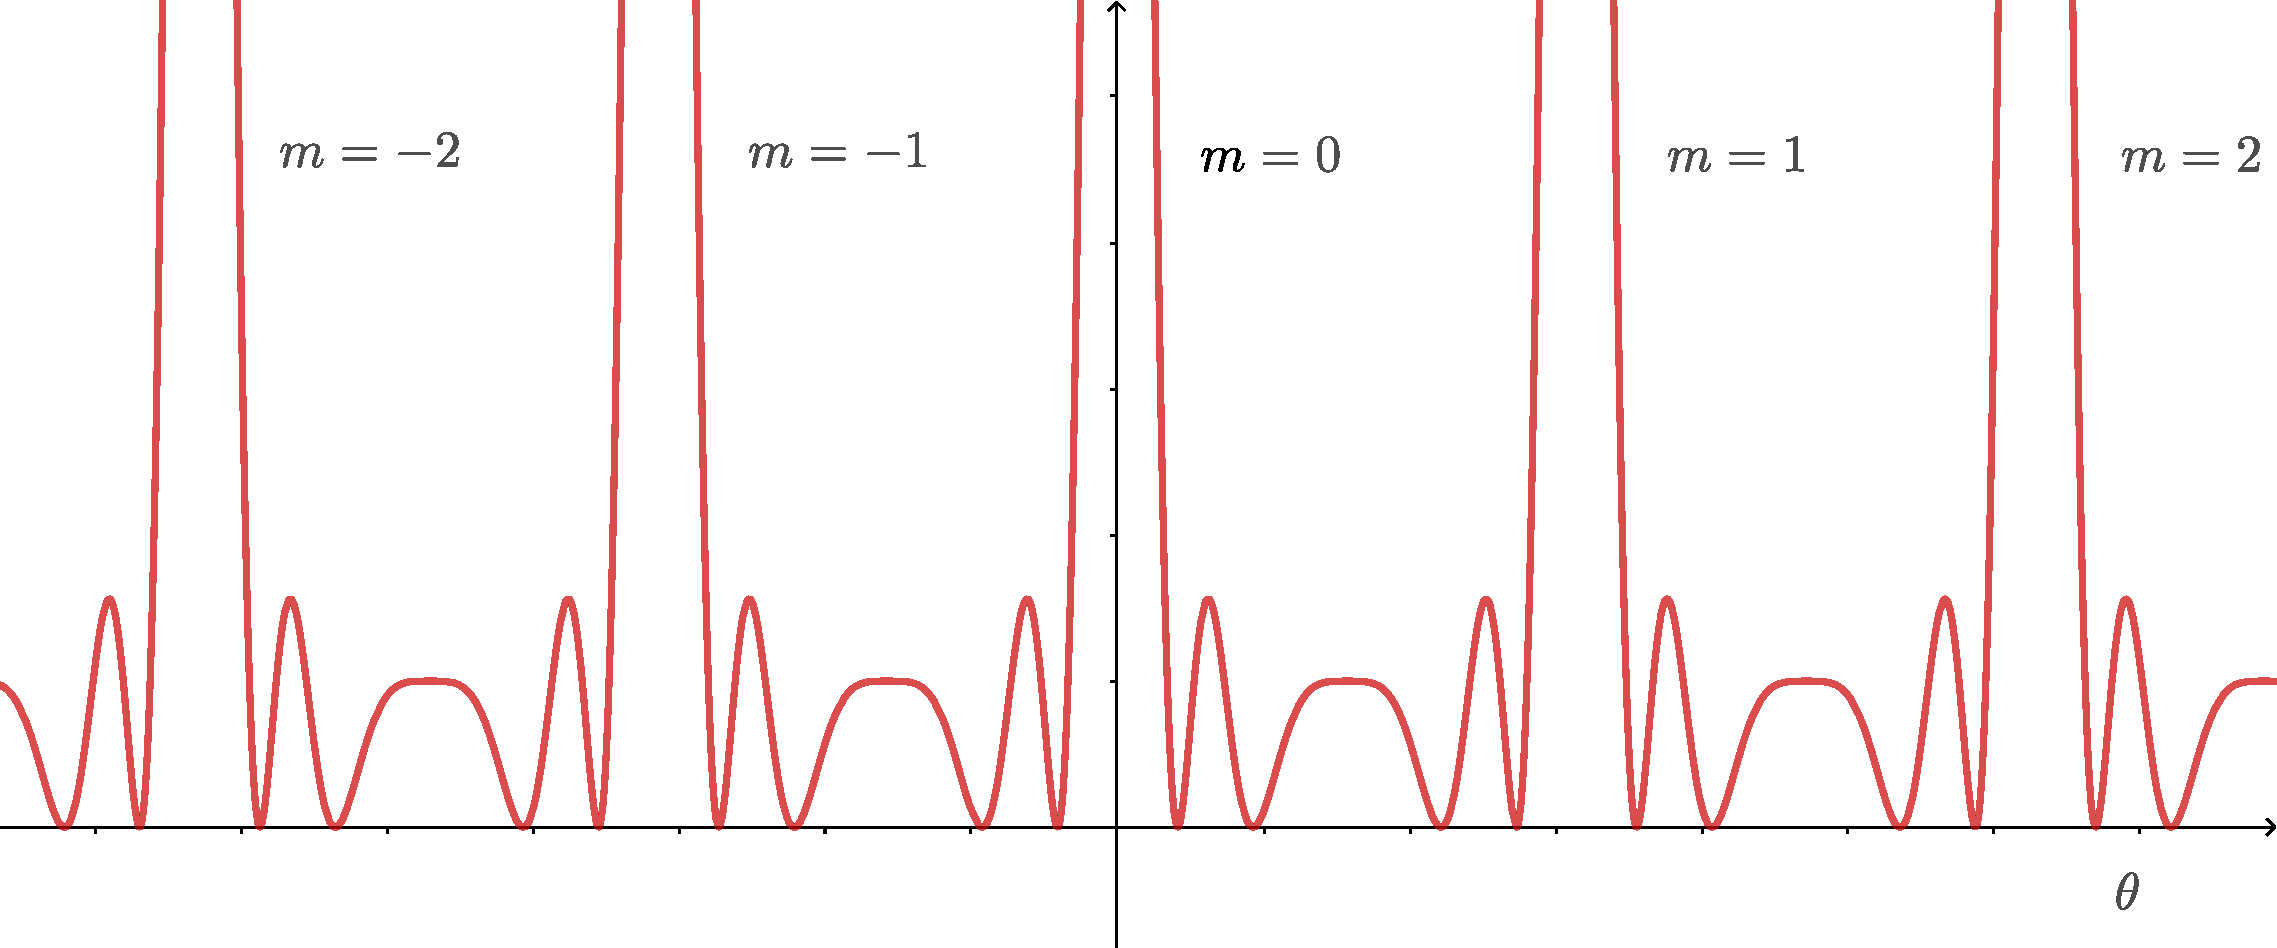
\includegraphics[width=0.8\textwidth]{fig/a2007_s6.pdf}
\end{center}
Let's proceed with finding the width of the $m=2$ maximum. You'll need to know that `width' means the distance between the two minima on either side of the maximum. These minima correspond to the instances of $\sin^2\left(\frac{N\Delta\varphi}{2}\right)=0$ which lie nearest to $\Delta\varphi=4\pi$. In that case $\Delta\varphi=4\pi\pm \frac{2\pi}{N}$, or $\sin\theta= \frac{2\lambda}{d}\pm \frac{\lambda}{Nd}$. These values for $\theta$, which we'll denote by $\theta_+$ and $\theta_-$, are very close. We seek their difference $(\theta_+-\theta_-)\equiv\Delta\theta$. Subtracting the sines, we find 
\begin{equation*}
	\sin{\theta_+}-\sin{\theta_-}=\frac{2\lambda}{Nd}=2\sin{\left( \frac{\Delta\theta}{2}\right)}\cos{\left( \frac{\theta_++\theta_-}{2}\right)}=\Delta\theta\cos{\theta}
.
\end{equation*}
Here $\cos{\theta}=\sqrt{1-\sin^2{\theta}}=\sqrt{1-\left(\frac{m\lambda}{d}\right)^2 }$, so
\begin{equation*}
\boxed{\Delta\theta = \frac{2\lambda}{N\sqrt{d^2-(m\lambda)^2}}=\ang{;0.184}.}
\end{equation*}

\end{solution}
\fi

\end{document}
